\documentclass[11pt,a4paper]{article}
\usepackage[]{fontspec}
\usepackage[brazil]{babel}
\usepackage{graphicx}

\title{Gerenciamento de Memória \\ {\small Roteiro da Aula Prática utilizando o SOsim~\cite{bib:sosimlab}}}
\author{Prof. Adriano J. Holanda}
\date{\today}

\begin{document}
\maketitle

\section{Política de busca de páginas}

No menu {\rm Opções$\rightarrow$Parâmetros do Sistema, aba Memória} é
possível especificar a {\rm Política de busca de páginas}. Este
parâmetro especifica se as páginas serão carregadas de forma {\rm
  antecipada}, quando o processo for carregado, ou se serão carregadas
sob demanda, ou seja, quando forem necessárias para o processo.

\begin{figure}[h]
  \centering
  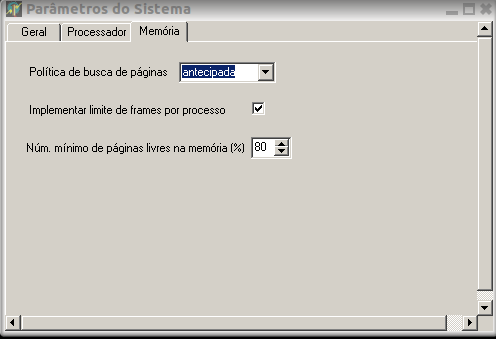
\includegraphics[scale=.45]{../img/sosim-parsys.png}
  \caption{Janela de entrada de parâmetros do sistema para a memória.}
  \label{fig:parsys}
\end{figure}

Se a política sob demanda for selecionada, na primeira requisição da
página haverá falha de página ({\em page fault}), pois a página ainda
não foi carregada na memória primária.

A memória do SOsim possui 100 {\em frames} de memória física.

\begin{figure}[h]
  \begin{minipage}[h]{.45\linewidth}
    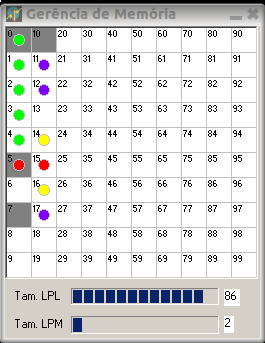
\includegraphics[scale=.575]{../img/sosim-mm.png}
  \end{minipage}
  \begin{minipage}[h]{.55\linewidth}
    \footnotesize
    \noindent FPL -- Lista de Páginas Livres ({\em Free Page List})\\
    \noindent MPL -- Lista de Páginas Modificadas ({\em Modified Page List})
  \end{minipage}
  \label{fig:mm}
  \caption{Janela de exibição do gerenciamento de memória.}
\end{figure}


\paragraph{Atividade.} Crie 2 processos limitados por processamento (CPU/bound).
No primeiro a política adotada para carregamento das páginas é a ``antecipada''.
Encerre o primeiro processo e altere a política de páginas para carregamento 
``sob demanda''. Verifique as diferenças entre as duas políticas, acompanhando 
os estados do bit de validade no PCB do processo em execução.

\section{Espaço de endereçamento}

\paragraph{Atividade.} Crie 2 processos CPU/bound com número de frames
diferentes. Verifique a alocação de memória para o espaço de endereçamento 
para cada processo e responda às questões: 

\begin{itemize}
\item Quais são os espaços de endereçamento mínimo e máximo?
\item Qual o tamanho da página virtual?
\end{itemize}

\section{Limite de frames e FIFO com buffer de páginas}

\paragraph{Atividade.} 

Ajuste os seguintes parâmetros:
\begin{enumerate}
\item Escalonamento: circular (Round-Robin);
\item Política de busca de páginas: sob demanda.
\end{enumerate}

Execute os seguintes passos:

\begin{enumerate}
\item Crie um processo CPU/bound com limite de 3 frames;
\item Ative a janela ``Contexto do Processo'' para visualizar a tabela
  de páginas do processo;
\item Observe na janela ``Gerência de Memória'' a alocação de frames.
\end{enumerate}

Tente responder às questões:
\begin{enumerate}
\item O que acontece quando a página 3 (quarta página) é requisitada?
\item E a página virtual 4?
\item O que acontece quando a página virtual 0 é requisitada novamente?
\end{enumerate}


\begin{thebibliography}{5}
  \bibliographystyle{plain}
\bibitem[SOsimLab]{bib:sosimlab} Arquitetura de Sistema
  Operacionais. Machado/Maia. Editora LTC, 4$^a$ edição. Capítulo 10
  –- Gerência de Memória Virtual.
\end{thebibliography}

\end{document}

\documentclass[a4paper,11pt]{article}

\usepackage[utf8]{inputenc}
\usepackage[brazil]{babel}
\usepackage{a4wide}

\def\sosim{{\sc SOsim}}
\def\cpu{{\tt CPU/bound}}
\def\io{{\tt IO/bound}}

\begin{document}
\begin{center}
 Trabalho de Sistemas Operacionais I\\
 Prof. Adriano J. Holanda\\
 FAFRAM, 6/11/2012\\
\end{center}
\noindent Nome:  \\
\noindent Nome: \\

\paragraph{Questão 1.} Realize os seguintes procedimentos: 
\begin{enumerate}
\item \label{init:demanda} Inicialize o \sosim{} com a política de
  busca de páginas {\tt sob demanda};
\item \label{cpu:demanda} Crie um processo \cpu{};
\item Ative a janela PCB para visualizar a tabela de páginas do
  processo (sempre realize este procedimento após a criação de um
  processo);
\item \label{desc:demanda} Descreva as alterações que ocorrem na tabela de
  páginas conforme o processo vai sendo executado com relação a falha
  de páginas ({\em page fault}) e alocação da memória real;
\item Finalize o processo;
\item Altere a política de busca de páginas para {\tt antecipada};
\item Crie um processo \cpu{};
\item Repita o procedimento do item~\ref{desc:demanda}.
\end{enumerate}

\paragraph{Questão 2.} Realize os seguintes procedimentos: 

\begin{enumerate}
\item Repita o procedimento~\ref{init:demanda} da Questão~1;
\item Crie um processo \io{};
\item Repita o procedimento~\ref{desc:demanda} da Questão~1,
  comparando as alterações na tabela de páginas (principalmente tempo
  entre a alocação das páginas) com o processo \cpu{} executado no
  item~\ref{cpu:demanda} da Questão~1;
\item Se houver diferenças entre os processo \cpu{} e \io{}, explique
  os motivos.
\end{enumerate}

\paragraph{Questão 3.} Realize os seguintes procedimentos: 
\begin{enumerate}
\item Crie um processo \cpu{} com limite de $3$ {\em frames} com
  política de paginação sob demanda e política de escalonamento
  circular ({\tt Opções$\rightarrow$Parâmetros do
    sistema$\rightarrow$Processador});
\item Descreva a sequência de alocação de memória acompanhando as
  alterações na tabela de páginas;
\item Quando os 3 {\em frames} estão alocados e há necessidade de
  alocação de mais 1 {\em frame}, qual a política adotada pelo
  gerenciador de memória para liberar o {\em frame} na memória real e
  qual é a alteração ocorrida na tabela de páginas.
\end{enumerate}

\vfill

\begin{flushright}
  {\Large Bom Trabalho.}
\end{flushright}

\end{document}
